\documentclass[tikz]{standalone}

\usepackage{tikz}
\usetikzlibrary{trees}
\usetikzlibrary{shapes}
\usetikzlibrary{positioning}
\usetikzlibrary{arrows.meta}

\tikzset{
    mynode/.style = {circle, ultra thick, draw=black, align=center,fill=yellow!30,font=\ttfamily\bfseries\Large,text=black},
    mynoder/.style = {circle, ultra thick, draw=black, align=center,fill=red!30,font=\ttfamily\bfseries\Large,text=black},
    mynodeb/.style = {circle, ultra thick, draw=black, align=center,fill=blue!30,font=\ttfamily\bfseries\Large,text=black},
    mynodeg/.style = {circle, ultra thick, draw=gray, align=center,fill=gray!05,font=\ttfamily\bfseries\Large,text=gray!20},
    mynodegr/.style = {circle, ultra thick, draw=gray, align=center,fill=gray!05,font=\ttfamily\bfseries\Large,text=red},
    edgen/.style = {-,ultra thick,black},
    edger/.style = {-,ultra thick,red},
    edgeb/.style = {-,ultra thick,blue},
    edgeg/.style = {-,ultra thick,gray},
    edgegd/.style = {-,ultra thick,brown,dashed}, % back
    edgevd/.style = {-,ultra thick,violet,dotted}, % forward
    edgexd/.style = {-,ultra thick,blue,densely dotted}, % traversal
    every picture/.style={/utils/exec={\ttfamily\bfseries}},
    every picture/.style={font issue=\ttfamily\bfseries},
    font issue/.style={execute at begin picture={#1\selectfont}}
}

\begin{document}

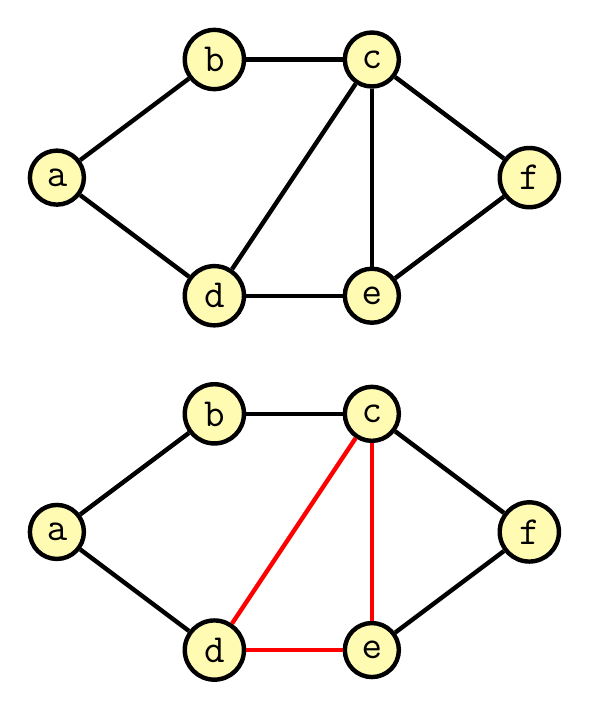
\begin{tikzpicture}[scale=1.00,transform shape]
\node[mynode] at (0,-4.5) (a2) {a};
\node[mynode] at (2,-3.0) (b2) {b};
\node[mynode] at (4,-3.0) (c2) {c};
\node[mynode] at (2,-6.0) (d2) {d};
\node[mynode] at (4,-6.0) (e2) {e};
\node[mynode] at (6,-4.5) (f2) {f};
%
\draw[edgen] (a2) edge node {} (b2);
\draw[edgen] (a2) edge node {} (d2);
\draw[edgen] (b2) edge node {} (c2);
\draw[edgen] (d2) edge node {} (e2);
\draw[edgen] (d2) edge node {} (c2);
\draw[edgen] (e2) edge node {} (f2);
\draw[edgen] (c2) edge node {} (f2);
\draw[edgen] (c2) edge node {} (e2);
%
\node[mynode] at (0,-9.0) (a3) {a};
\node[mynode] at (2,-7.5) (b3) {b};
\node[mynode] at (4,-7.5) (c3) {c};
\node[mynode] at (2,-10.5) (d3) {d};
\node[mynode] at (4,-10.5) (e3) {e};
\node[mynode] at (6,-9.0) (f3) {f};
%
\draw[edgen] (a3) edge node {} (b3);
\draw[edgen] (a3) edge node {} (d3);
\draw[edgen] (b3) edge node {} (c3);
\draw[edger] (e3) edge node {} (d3);
\draw[edger] (d3) edge node {} (c3);
\draw[edgen] (e3) edge node {} (f3);
\draw[edgen] (c3) edge node {} (f3);
\draw[edger] (c3) edge node {} (e3);


\end{tikzpicture}

\end{document}